
\documentclass{beamer}
%
% Choose how your presentation looks.
%
% For more themes, color themes and font themes, see:
% http://deic.uab.es/~iblanes/beamer_gallery/index_by_theme.html
%

% Theme License: https://creativecommons.org/licenses/by/4.0/

\mode<presentation>
{
  \usetheme{metropolis}   % https://github.com/matze/mtheme
  \usecolortheme{default} % or try albatross, beaver, crane, ...
  \usefonttheme{default}  % or try serif, structurebold, ...
  \setbeamertemplate{navigation symbols}{}
  %% \setbeamertemplate{caption}[numbered]
  \setbeamertemplate{caption}{\raggedright\insertcaption\par}
}

\usepackage[english]{babel}
\usepackage[utf8x]{inputenc}
\PassOptionsToPackage{hyphens}{url}\usepackage{hyperref}

\title{Data Privacy}
\author{Jake Vossen}
\institute{Colorado School of Mines - ACM-W}
\date{TODO}

\begin{document}
\begin{frame}{Something to consider...}
  \begin{figure}
    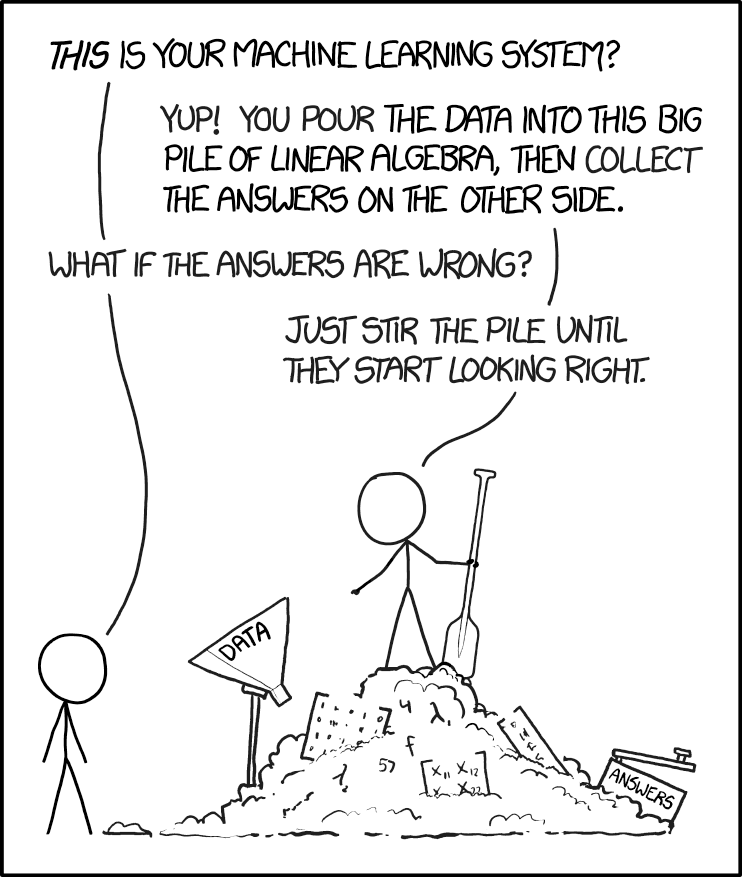
\includegraphics[scale=.18]{machine_learning_2x.png}
    \caption{https://xkcd.com/1838/}
  \end{figure}
\end{frame}
\begin{frame}
  \titlepage
\end{frame}

% Uncomment these lines for an automatically generated outline.
%\begin{frame}{Outline}
%  \tableofcontents
%\end{frame}

\begin{frame}[fragile]
  \frametitle{What does the topic of data privacy include?}
  \begin{itemize}
    \item Personal data protection
    \item The ethics of collecting user data, and the impacts it has on society
    \item Data protection technologies, such as encryption and it's various applications
    \item Legislation regarding data protection (ex GDPR), and regulations on encryption
  \end{itemize}
\end{frame}

\section{Why \textbf{you} should care about data privacy}


\end{document}
